\documentclass[a4paper,11pt]{article}
\usepackage{fullpage}

\usepackage[utf8]{inputenc}
\usepackage[british]{babel}

\usepackage{amsmath}
\usepackage{amssymb}
\usepackage{amsthm}
\usepackage{color}
\usepackage{float}
\usepackage{listings}
\usepackage{fontenc}
\usepackage{graphicx}
\usepackage[hidelinks]{hyperref}

\usepackage{multirow}


\title{\textbf{Human Computer Interaction 5 C (Course 1MD016) \\
    Uppsala University -- Spring 2015 \\
    Report for Expert Evaluation}}

\author{
Philip \AA kerfeldt\\
\textup{Dept. of Information Technology}\\
\textup{Uppsala University}\\
\textup{Uppsala Sweden}\\
\textup{Philip.Akerfeldt.4987@student.uu.se}
}


\date{\today}

\begin{document}
\maketitle
\newpage
\tableofcontents
\pagebreak


\section{Scenario}
To analyse the redesigned system a scenario was chosen in with regard to user group that the designers chose and the guide on how to create scenarios in chapter three of the book \textit{Designing Interactive Systems} by David Benyon \footnote{Benyon D., Turner P. and Turner S. (2005). Designing Interactive Systems. Essex, England: Pearson Education Ltd \\
Page: 56-57}.\\ 
The chosen scenario can best describes as a conceptual one with a "typical" persona acting in it. The scenario at hand is carefully derived from the previously written parts of the report describing the typical user and their intentions in using the system. The intention I'm referring to is of course the planning of booking tickets to a movie and then actually realizing the booking and/or purchase of the ticket/tickets.\\

When choosing persona that will act in the scenario it was somewhat derived from the previously written parts of the report describing the user groups of the system and their goals. The persona in this case is a person who has a fundamental experience when it comes to handling computers and the internet. \\
A persona that fits this description is Vladimir, 20, who is a technological student at KTH university in Stockholm. He was born and raised in Kiev so naturally his mother tongue is Ukrainian but he knows quite a lot of swedish but it's far from perfect. Since he is studying technology at KTH he is used to handling different systems and webages in general. Vladimir is sitting at home and has nothing to do so he decides that he wants to see a movie a few hours later that night. In his own pace and without disturbance he intends to use the webpage \url{www.sf.se} to reach his goals of finding a suitable movie and going through with the reservation of the movie at hand. He uses his own laptop to carry out the reservation. \\    
		

\section{Hierarchical Task Analysis}

\begin{figure}[H]
\centering
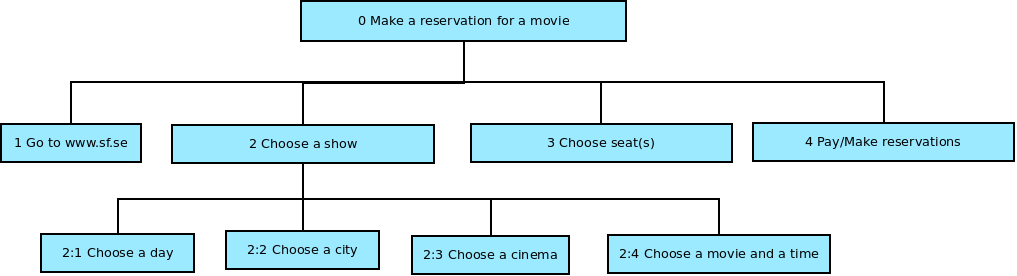
\includegraphics[scale=0.5]{Diagram1.png} 
\caption{HTA}
\end{figure}

\newpage
\section{Streamlined Cognitive Walkthrough}

\begin{enumerate}
\item This step is quite trivial in my opinion since the Vladimir will instantly recognize if he has arrived at the right web page or not and will therefore know if he can proceed in order to achieve his goal. No confusion should erupt at this at all and a clear path of progress should have been created by Vladimir.

\item When the Vladimir clicks the button \textit{"Biljetter"} he will, when the page updates, have four choices to do in order to make a reservation for a film. Three of the choices are from separate roll-down (curtain) menus.\\ 
The first choice he needs to do is to choose a day for which he wants to see the movie. When the choice has been made the list of movies shown below are updated so there should be no confusion of whether the action was correctly done or not.\\
The second choice \underline{must} be of the city in which he want to see the movie. This is because the third choice which is the cinema depends on which city was chosen. This is because every city has a specific number of cinemas and they all have unique names. The redesign is not cristal clear about the order of the roll-down menus so this can be confusing for Vladimir.\\
When this has been done he is presented with two choices; either choose a movie directly from the filtered list below if he doesn't care about which cinema he watches it in. If this is done he will be presented with a list of the cinemas that shows this specific movie and some other information related to this show. Since the page automatically changes he should not have any problems with knowing what to do next.\\
The second choice is if he, however, does care about which cinema he watches the movie in. Then he needs to specify this in the third roll-down menu.\\
The last two choices he could do could possibly present some confusion since there is not a clear path of action. This is because you can, after the second choice (city), continue on two different paths in order to choose a show.
 
\item 
When Vladimir arrives at this step it should be pretty straight forward since the graphical design and overall layout makes it hard to be confused. He can choose the number of seats he want the reservation to be for and where in the cinema he wants to sit. When he chooses the number of seats he wants the reservation to be for they are displayed as white boxes on the 2D model of the cinema. Already booked seats blinks white twice and are later marked with red. If he was to move his seats over the already booked ones his will be marked with red crosses that indicate that this action cannot be performed. When he has chosen the seats in the cinema they stick to the 2D model letting him know that the action was correctly performed. 

\item 
At this step the choices that can be made are very clear and there should not be any confusion from Vladimir’s point. He is presented with two choices; either he buys the tickets and should therefore fill in the empty boxes belonging to that option. Or he could make a reservation for which he needs to do the same thing except in the box for reservation instead of purchase. 

\end{enumerate}

\newpage
\section{Heuristic Evaluation}

\subsection{Visibility of system status} 
When a user starts a reservation process through the system the user will be presented with an overlaying "progress"-bar which shows the user numbered boxes with names of the steps in the progress. This is done by making the text of the step the user is currently on bold and black and also making the number of the step in a yellow circle. Something that also enhances this sensation is that the other steps have a greyish color of their font. When the user is done with a step and has moved on the new step will be highlighted (bold text and coloured number) whereas the previous step will be "faded" (greyish font colour) with their number in a green circle which indicates that the step is done.

\subsection{Match between system and the real world}
The language that the site uses is easy to handle for users that have been to a cinema before or if they have made purchases online before. The second situation only applies if the user wants to actually buy the tickets in advance. \\
They layout of the site is easily recognizable with the classic menu at the top and the typical order in which you should perform a series of tasks. The site should be read and navigated as you would read a newspaper or a book; from top right to bottom left. This layout should be easy for the user, with previous internet experience, to adapt to when visiting the site. 

\subsection{User control and freedom}
The site does not provide the user with clear options to return to a page they can recognize if they by mistake navigated somewhere they didn't mean to. The user can click on the company’s logo in the top-bar menu in order to get to the front page of the site. Besides that the user can almost all the time use the top-bar menu to navigate to a certain page of the site. Since the current location is highlighted in the top menu with a yellow colour whereas the other headings are white. 
If the user is not familiar with the site at all the user can always use the browsers navigation arrows to go forwards or backwards on the site.

\subsection{Consistency and standards}
The layout of the new design uses a words and titles for their different section that are separable. There is also a consistent difference between cinema-related sections and commercial sections. 

\subsection{Error prevention}
The layout and design prevents errors with the help of error-messaging for example. The site also prevents the user to skip steps when a reservation is being performed. Another example of when the site prevents errors is when you are supposed to choose a day, cinema, city etc. If the user do not choose a day for example but instead moves directly on to choosing a movie the user cannot move on without specifying the cinema and city. 

\subsection{Recognition rather than recall}
During an ongoing reservation there is a summary of the choices made so far in the top right corner. Information is added to this box when they have been done during the reservation. This way of showing information along with the information from the progress-bar that was discussed earlier make the user aware of the information that was chosen. 


\subsection{Flexibility and efficiency of use}
The site offers multiple ways of making reservations that are different when speaking of the level of difficulty. This is because of the different graphical representations in the different ways of performing a reservation. Whether these different ways of performing a reservation are faster or slower than each other, in proportion to the level of expertise of the user, is hard to determine without a proper analysis with multiple users with different experience of the system.

The way the system is designed at the moment a very experienced user probably wont find it as optimized as it could be. The pros of this layout design is the broad spectrum of user that it can appeal to. The more experienced users will be able to use the system without any problems at all and the less experienced users can still navigate around the site and achieve their goals within a certain time frame.   

\subsection{Aesthetic and minimalist design}
The site as it is designed now contains a lot of information spread out on the site. This can be confusing for the user since the focusing on the planned task can become hard. The new design didn’t change that much about the layout besides stripping some features down and adding some minor features to the current design. The stripping of features was fairly good in a sense that it was aimed to ease the process for the user. The negative parts of this will be discussed in a section below. 

\subsection{Help users recognize, diagnose, and recover from errors}
The error messages that the page delivers when the user encounters problems are minimal and simplistic. An example of this can be when the user is at the stage called "V \"a lj Platser" where the user is expected to choose seats in the cinema. If the user have not chosen any seats and tries to continue to the next step a small box will pop up above the button telling the user that he/she needs to choose seats before continuing. The box could have been a little bit bigger but the design it has now matches the overall design of the current site which is minimalistic and clean. 

\subsection{Help and documentation}
If the design doesn't help the user as much as it should the user can always use the search box in the top right corner to search for the thing they want help with. When the search query has been performed the given results are shown under different titles to help the user understand the results.\\
If the user doesn't use the search box there is always the Q\&A at the bottom of the page that shows the most common questions asked and the answers to them. The questions are also sorted under different titles making a search for a specific question a bit easier.

\newpage
\section{Think Aloud}
I performed a "Think Aloud"-interview with a 22 year old male who has a very good experience of computers and websites over all which makes him a good candidate considering the previous parts of the design report. Before the interview began the task of ordering 2 tickets to a specific movie was given to the interviewee. 
The first thing he commented was the difficulty of the interview. His opinion was based on the fact that the interviewer had to describe all the changes that were done and show the pictures that were attached to the report in order for him to understand the changes that were made. He said that it was strange that he had to ask the interviewer for descriptions since he didn't want to read a major part of the report in order to perform a \textit{Think Aloud} interview.

When he was presented with the first design proposal he thought that it was not really necessary to change the design. He explained this by saying: \textit{"If I navigate myself to the header called "Cinemas" i probably want information about the cinemas specifically and not the movies that are being shown there"}.

To change the colours of the headlines of the different section on the front page wasn't such a bad idea according to him and he thought it would be such an easy thing to simplify on the front page that it would be bad not to do it.

When he came to the stage of making the reservation he was presented with the picture of the redesign and he instinctively commented that it was strange to add the curtain-menu "V\"alj stad" lastly since one of the other menus depend on the choice made in that certain menu. When the interviewer explained that the picture was misleading and the caption to the text explained that the menus "V\"alj biograf" and "V\"alj stad" would be switched he commented that it would probably have made more sense to do that in the picture in the first place. But over all he thought that it was a really good feature and that the designers made some really good points in the section.

When he came to the stage of choosing seats he said that it was really good that they removed the grey arrows in the 2D model of the cinema since they didn't really say anything according to him. The choice of removing the counter for remaining time was not so good according to him. He understood how the designers were thinking but gave the idea that instead of removing the counter entirely you could just increase the time. His justified his idea by saying that he would probably have been confused if the page all of a sudden refreshed. He said that he would have become angry because he would not have understood what just happened.

%\newpage
%\section{Ethical Analysis}
%The design of the website as it is now is pretty limited to a certain group of people. That group of people can best be describes as Swedish people without disabilities. The current limitation is because of the information regarding for example possibilities for disabled people to watch a movie or if you are English speaking. There are information regarding these issues but they are not automatic or well displayed. You can for instance find information concerning the possibility for disabled individuals to watch a movie. In order to do this you need to be in the page where you choose your seats and then click the title, below the 2D model, which is called \textit{"L\"as mer om Salongen"}.

%If you are speaking another language than Swedish you don't really have a choice that will ease the process of reserving tickets. If you are using for example Google Chrome with certain settings the browser can translate the page for you which works fairly good to be honest. This makes it even harder to find reasons not to implement this right away. The fact the English speaking users are a fairly small group doesn't really justify the sites current design and it should be changed as soon as possible.

\newpage
\subsection{Ranking Of Usability Problems}
The current design of the website is actually quite good and this can be shown by the few details that the designers of the new system changed in order to make the old system better. The big menu-bar at the top of the page is something critical to be able to navigate the system easily and this could be altered in a small way perhaps but never removed entirely or changed drastically. The color choices of the page should not be altered either since they contribute to a comforting feeling and are warm without making the user lose their focus on the important parts. If the group would like to change the figure that represents the page when the user have pressed "Boka biljetter" so that it shows the actual order of the roll-down menus that would simplify matters a lot. Note that this is not a problem but a minor fix that would eliminate confusion and that it can also be fixed by explaining the arrow in the text instead of the figure caption.  

\textbf{Major Problems}
A big problem is where the site currently wants the user to focus. For instance when making reservations for a movie when the user has chosen a movie. The page that is shown when this is done lacks focus on what really matters. The user probably wants it to be clear what movie he/she chose. This information is currently being displayed as a quite small picture with some information besides it. An enlargement of this would perhaps assists the user in focusing on the right things on the page. 

\textbf{Minor Problems} 
The front page of the site could still be a lot clearer with all the commercials that consume a lot of the users focus. A slight compression of the commercials and enhancement of the movie-related section would make the front page a lot less ungainly.

\section{Reflection}
The method I used that I found to be the most efficient in order to evaluate this specific system was the Heuristic Evaluation (HE). This was because the method gave me some really useful tools in order to analyse and evaluate the system effectively. There was a clear template to follow which made the step-by-step process of evaluation really comfortable and easy. The Streamline Cognitive Walkthrough (SCW) also had its benefits but lacked the depth that was achieved when using the HE.

A note that should not be neglected was the lack of a clickable redesign which made the process somewhat difficult and most certainly slower than if a clickable prototype would have been supplied.

\section{Sources}

\begin{enumerate}
\item Benyon D., Turner P. and Turner S. (2005). Designing Interactive Systems. Essex, England: Pearson Education Ltd\\

\end{enumerate}

\end{document}